\section{Linear Regression Model}

\subsection{One hot encoding}

Linear regression can only operate on numerical values. This caused an issue with the \textbf{Sex} column as it is not numeric. I had to use a technique called "one hot encoding" to transform the Sex column into a usable feature. Interestingly, one hot encoding does not merely transform the sex column into 1 for infant, 2 for male, 3 for female. Instead it creates three new features. These new features are F for female, I for infant and M for male. The feature can have a value of either 1 or 0, 1 meaning "is a" and 0 meaning "not a". For example if F has a value of 1 then we can say it is a female. Alternatively if F has a value of 0 then we can say it is not a female. The results can be seen in figure \ref{fig:abalone-one-hot-encoding}
\begin{figure}[H]
  \centering
  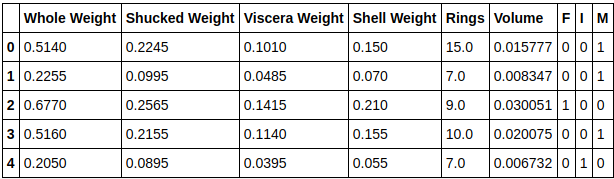
\includegraphics[scale=0.5,width=100mm]{./images/abalone-one-hot-encoding.png}
  \caption{Table showing the results of one hot encoding}
  \label{fig:abalone-one-hot-encoding}
\end{figure}

\subsection{Linear Regression}

\begin{figure}[H]
  \centering
  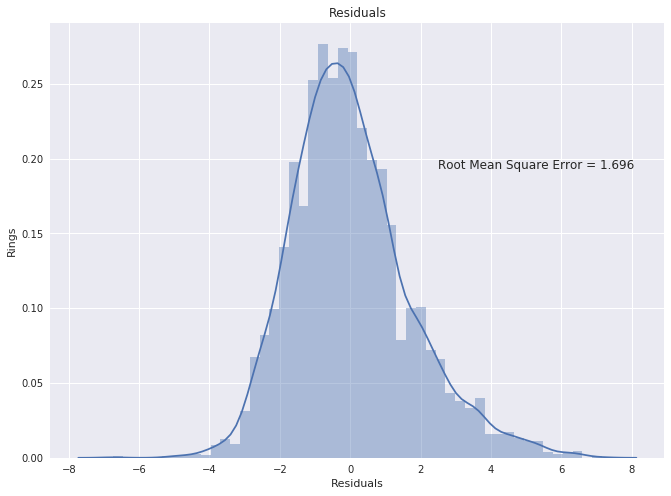
\includegraphics[scale=0.5,width=100mm]{./images/abalone-linear-regression-hist.png}
  \caption{Root mean squared error of  our linear regression}
  \label{fig:abalone-linear-rmse}
\end{figure}

Figure \ref{fig:abalone-linear-rmse} shows a distribution of our residual errors. The residuals seem to follow a fairly normal distribution and our root mean squared error is not bad at 1.69. However our regression score comes out as 0.49. This means that our model will only be correct around 50\% of the time. This is not great.
\begin{figure}[H]
  \centering
  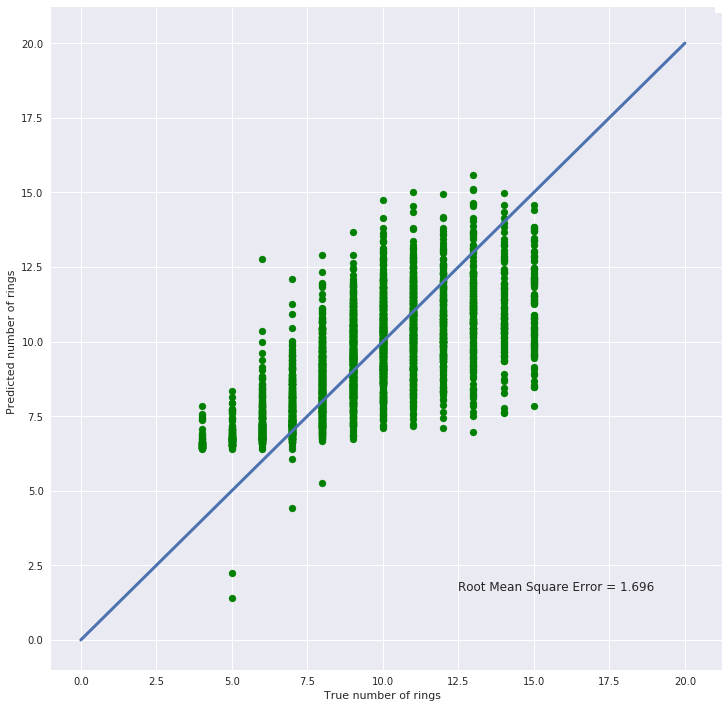
\includegraphics[scale=0.5,width=100mm]{./images/abalone-linear-regression-line.png}
  \caption{Linear regression line for predicting the age of abalones based on the rings}
  \label{fig:abalone-linear-regression-line}
\end{figure}
Figure \ref{fig:abalone-linear-regression-line} shows the linear regression line. From a quick glance the model does not seem to fit our expected value very well. There is a possibility that the sex column may be throwing things off. I shall try plotting a linear regression for each sex. 

\begin{figure}[H]
  \centering
  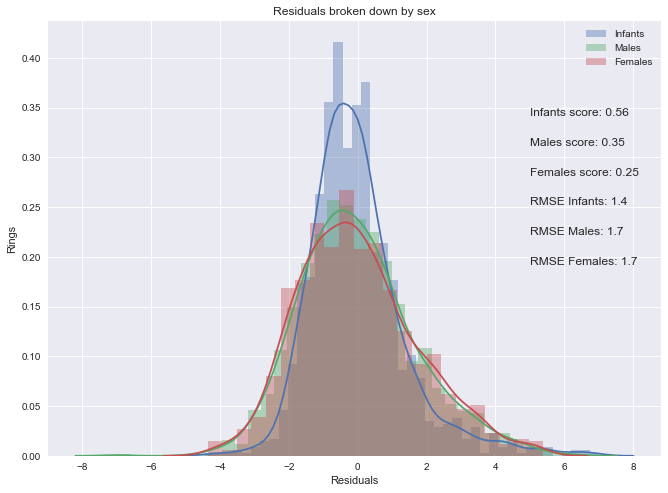
\includegraphics[scale=0.5,width=100mm]{./images/abalone-linear-regression-hist-sex.png}
  \caption{Residuals for values broken down by sex}
  \label{fig:abalone-linear-regression-hist-sex}
\end{figure}

Figure \ref{fig:abalone-linear-regression-hist-sex} seems to indicate that breaking down the values into different sexes does improve the RMSE and the regression score for the infants. However for both male and female our prediction and RMSE seems to have gotten worse. The overall results though are disappointing as 56\% still is not great. Lets check the residuals versus each feature to see if there is any particular feature which may be skewing our results.
\begin{figure}[H]
  \centering
  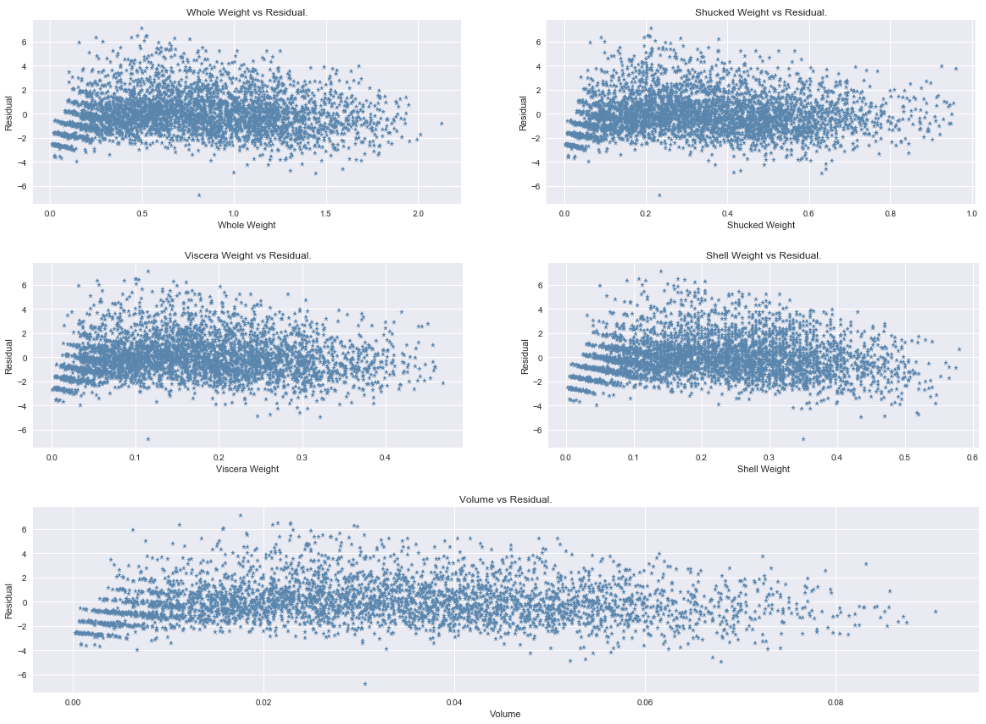
\includegraphics[scale=0.5,width=100mm]{./images/abalone-residuals-vs-features.png}
  \caption{Residuals VS all features}
  \label{fig:abalone-residuals-vs-features}
\end{figure}
The scatter plots seem to indicate that the values are not normally distributed. This means that there may be higher order features that are not accounted for. If this is the case then a linear regression model wont be able to make an accurate prediction. 

\subsection{Lasso Regression}

Lets see if we can improve things using lasso. Lasso is a regression analysis method that performs variable selection and regularization to try and improve accuracy.
\begin{figure}[H]
  \centering
  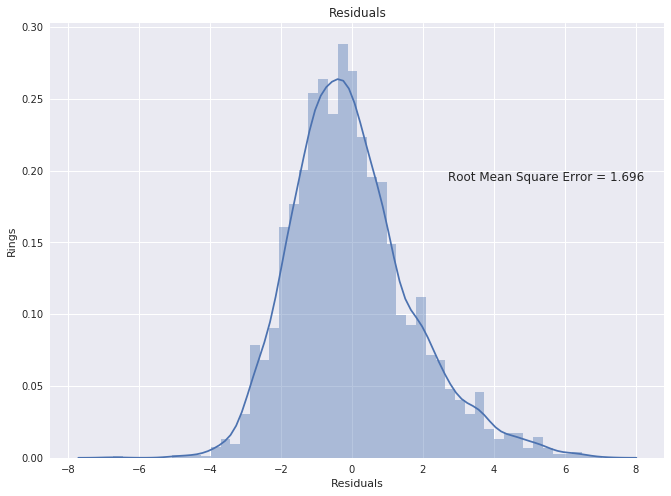
\includegraphics[scale=0.5,width=100mm]{./images/abalone-lasso-regression.png}
  \caption{Root mean squared error for lasso regression}
  \label{fig:abalone-lasso-regression}
\end{figure}
Figure \ref{fig:abalone-lasso-regression} shows that lasso marginally improves our RMSE score. It improves it by 0.001 to be exact. 
\begin{figure}[H]
  \centering
  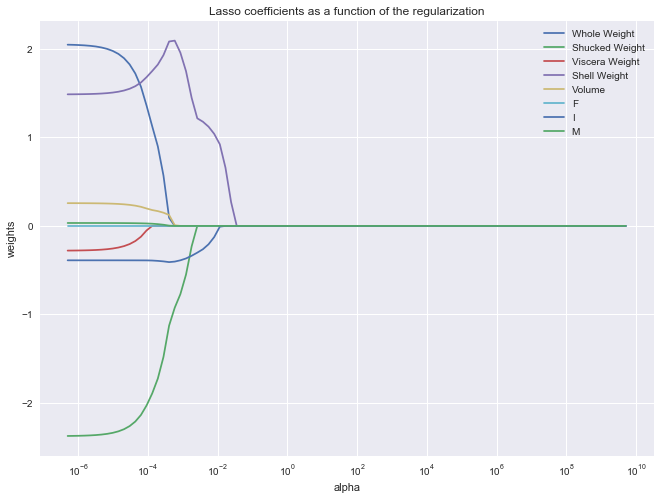
\includegraphics[scale=0.5,width=100mm]{./images/abalone-lasso-plot.png}
  \caption{Lasso coefficients as a function of the regularization}
  \label{fig:abalone-lasso-plot}
\end{figure}
Figure \ref{fig:abalone-lasso-plot} shows the lasso plot displaying each coefficients importance towards the predictor. From the plot, we can see that whole weight has a very little bearing on the outcome as it dips towards zero very fast. Shell weight and infant type abalones seem to be the most important of our coefficients. Our lasso regression score, however, remains similar our linear regression score at about 49\% accuracy. I tried tuning the alpha parameter for maximum effect by tuning some of the hyper-parameters using GridSearchCV, however, this was not very successful and only marginally improved the score by a fraction of a percentage.

\subsection{Ridge Regression}

\begin{figure}[H]
  \centering
  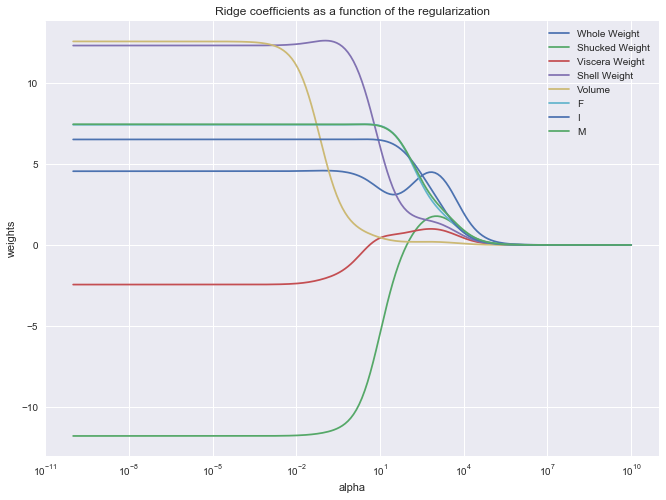
\includegraphics[scale=0.5,width=100mm]{./images/abalone-ridge-regression.png}
  \caption{Ridge coefficients as a function of the regularization}
  \label{fig:abalone-ridge-plot}
\end{figure}

Figure \ref{fig:abalone-ridge-plot} shows the ridge plot showing each coefficients weight towards the predictor. Both viscera weight and volume seems to collapse quite quickly towards zero indicating they do not have much bearing on the predictor. Infant, Male and Female seem to be the last to hit the zero spot which could mean they have good weights towards the predictor. Similar to lasso regression in figure \ref{fig:abalone-lasso-plot} Whole weight looks like a good coefficient towards the predictor. 

Unfortunately, the ridge score performed similarly to both linear regression and lasso regression in that it comes to 49\% accuracy. Again I tried tuning the hyper-parameters with GridSearchCV but changing the alpha had a very little effect on the outcome. The RMSE for ridge regression performed worse than lasso with a value of 2.8044.

After going through 3 forms of regression with 49\% accuracy it is clear that there is something wrong with our data as it does not seem to be a good fit for linear regression. Perhaps some data is missing, such as geographical locations or environmental conditions.